
\documentclass[PICOReport.tex]{subfiles}

\begin{document}

\comblue{Let's make clear that there are numerous signals that need to be separated; rather than a 'signal' and 'foregrounds'.} 
Contamination of CMB observations by astrophysical foreground emission of various origins is one of the major challenges that future observations of CMB polarization must face. Polarized emission in the PICO frequency range is known to be dominated by synchrotron emission from the galactic interstellar medium in our own galaxy and by thermal emission from interstellar dust. Although much has been learnt about these polarized foregrounds with WMAP and Planck observations, their exact properties are not known at the level that would be needed to guarantee that they can be separated out from the CMB using known component separation techniques. In particular neither the exact form one should assume for the frequency scaling of their emission (if any), nor the variation of these emission laws across the sky or along the line of sight, nor the small-scale distribution of emission, are known at the required level of detail. Whether other processes emit at a level that can contaminate PICO observations significantly is also not known at present. 

The many frequency channels of PICO can be used to learn from the PICO observations themselves the properties of these foregrounds, and to identify the CMB contribution in the multifrequency data using its unique spectral signature. To be robust against our uncertainty about the foregrounds, we assess the feasibility of foreground cleaning for different models of foreground emission of varying complexity, from optimistic to pessimistic, and for various component separation methods. 

%%%%%%%%%%%%%%%%%%%%%%%%%%%%%%%%%%%
\subsubsection{PSM sky simulations at $\boldsymbol{N_{\rm side}=16}$}
%%%%%%%%%%%%%%%%%%%%%%%%%%%%%%%%%%%

The PSM (Planck Sky Model) \cite{delabrouille/etal:2013} is a simulation software developed by the \emph{Planck} Collaboration  to model sky emissions at submillimetre to centimetre wavelengths based on the state-of-the-art observations of the \emph{Planck} satellite mission and earlier surveys. We use the {\sc PSM} to simulate all-sky polarization maps at the 21 frequency bands of \emph{PICO} ($21$ to $800$\,GHz). The simulated components of emission include CMB E- and B-mode polarization, polarized Galactic synchrotron and thermal dust foreground emissions. The CMB template map is generated from CAMB \cite{Lewis/etal:2000} through CMB E- and B-mode power spectra by assuming an optical depth to reionization of $\tau=0.06$ and a tensor-to-scalar ratio of $r = 10^{-3}$, as well as gravitational lensing effects. Galactic dust Q and U polarization maps are generated from the \emph{Planck} {\sc GNILC} 
dust intensity all-sky map at $353$\,GHz , in which cosmic infrared background (CIB), CMB, and noise have been filtered out, and assuming average polarization fractions of $5$-$10$\%. Galactic synchrotron Q and U maps are based on the \emph{WMAP} polarization observations at $23$\,GHz~\cite{Miville-Deschenes/etal:2008}. 

The thermal dust Q and U template maps are extrapolated across \emph{PICO} frequencies through a modified blackbody energy spectrum having variable spectral index and temperature over the sky, using the Planck {\sc GNILC} dust spectral index and temperature maps for which ${\beta_d = 1.6\pm 0.1}$ and ${T_d=19.4 \pm 1.3}$\,K, respectively. The synchrotron Q and U template maps are extrapolated across \emph{PICO} frequencies through a curved power-law spectrum, with a variable spectral index over the sky of ${\beta_s = -3\pm 0.06}$ based on the synchrotron index map from \cite{Miville-Deschenes/etal:2008}, and a constant curvature of $C_s = 0.3$ \cite{Kogut/etal:2007} to account for different populations of cosmic ray electrons  and possible AME polarization \cite{dickinson/etal:2018}. The CMB, dust, and synchrotron component maps in each \emph{PICO} frequency are then co-added, and instrumental white noise is added to each sky map using the sensitivities per frequency quoted by \emph{PICO}.
The PSM simulations are generated at a pixel resolution of HEALPix \cite{gorski/etal:2005} $N_{\rm side}=16$ ($2 \leq \ell \leq 47$), therefore assuming spectral variations of the foregrounds across $N_{\rm side}=16$ pixels.

%%%%%%%%%%%%%%%%%%%%%%%%%%%%%%%%%%%
\subsubsection{ PICO forecasts with \textsc{Commander}}
%%%%%%%%%%%%%%%%%%%%%%%%%%%%%%%%%%%

We have applied the \textsc{Commander} algorithm \cite{eriksen/etal:2008} to the set of PSM $N_{\rm side}=16$ sky simulations for \emph{PICO}.
\textsc{Commander} is a Bayesian parametric fitting method which has been thoroughly used by the \emph{Planck} Collaboration for the separation of CMB and foreground components \cite{Planck_2015_X,Planck_2018_IV}. Using MCMC Gibbs sampling in each pixel, the \textsc{Commander} algorithm allows to fit simultaneously the amplitudes of CMB and foreground components, their spectral parameters, and the CMB E- and B-mode power spectra in a self-consistent Bayesian framework. A Blackwell-Rao estimator applied to the Gibbs samples allows in particular to reconstruct the statistical (chi-square) distribution of the CMB B-mode power spectrum at each multipole, and the posterior distribution of the tensor-to-scalar ratio \cite{Remazeilles/etal:2016,Remazeilles/etal:2018}. Such a Bayesian method performs end-to-end propagation of all foreground uncertainties towards the tensor-to-scalar ratio, while providing a chi-square goodness-of-fit in each pixel which allows to revise the parametric model or readjust the galactic mask a posteriori. The \emph{PICO} sky maps are processed by \textsc{Commander} using a Galactic mask leaving a $50$\% fraction of the sky, and forecasts on $r$ are computed using the range of low multipoles $2 \leq \ell \leq 47$.

First considering \emph{PICO} sky simulations \emph{without foregrounds}, but just CMB and noise in the \emph{PICO} frequency bands,  we recover the tensor-to-scalar ratio with ${\sigma(r = 10^{-3}) = 0.40 \times 10^{-3}}$ significance: this provides the minimum uncertainty on ${r = 10^{-3}}$ that can be achieved by \emph{PICO} from low multipoles $2 \leq \ell \leq 47$ in the absence of foregrounds on $50$\% of the sky. In the presence of foregrounds (full simulation), with variable spectral indices over the sky, the \textsc{Commander} results on $r$ are of similar quality due to the broad frequency range of \emph{PICO} ($21$ -$800$\,GHz), with ${\sigma(r = 10^{-3}) = 0.41 \times 10^{-3}}$ for \emph{PICOv2-1.4} and ${\sigma(r = 10^{-3}) = 0.36 \times 10^{-3}}$ for \emph{PICOv3} (increased sensitivities per channel) after foreground cleaning. Assuming now that $60$\% delensing in power has been achieved (modified PSM simulation with only $40$\% of the lensing B-mode power left in the CMB map realisation), the uncertainty on ${r=10^{-3}}$ is improved by more than $30$\%, with ${\sigma(r = 10^{-3}) = 0.24 \times 10^{-3}}$ for \emph{PICOv3}  after foreground cleaning and $60$\% delensing. Finally, we note that discarding low- and high-frequency bands, resulting in a descoped version of \emph{PICO} with a narrower frequency range of $43$-$462$\,GHz, the \textsc{Commander} results are degraded by $75$\%, with an uncertainty  increasing from 
${\sigma(r = 10^{-3}) = 0.4 \times 10^{-3}}$  to ${\sigma(r = 10^{-3}) = 0.7 \times 10^{-3}}$ after foreground cleaning. The main reason for the degradation is a lack of constraining power on the dust temperature variations over the sky when discarding frequencies above $462$ GHz, which translates into a degradation of the fitted CMB B-mode power spectrum by extrapolation towards central frequencies. 
\newline\textcolor{red}{[MR: I can add a figure on \textsc{Commander} $C_\ell^{BB}$ results with \emph{PICO}, if needed]}

We are working in parallel on \textsc{Commander2}, a new version of the algorithm operating in harmonic space, thus allowing to perform the parametric fit at full resolution and to further reduce the uncertainty on $r$ by the increase of information / modes.


%%%%%%%%%%%%%%%%%%%%%%%%%%%%%%%%%%%
\subsubsection{Needlet analyis of PICO simulations}
%%%%%%%%%%%%%%%%%%%%%%%%%%%%%%%%%%%

The NILC is based on Internal Linear Combinantion (or ILC in short) component separation method. It has been applied to the PICO simulations to determine the angular power spectrum of the B-mode polarized CMB signal. This method only attempts to reconstruct the CMB signal, without using any prior information about foregrounds. It is based on two specific assumptions. Firstly, that the CMB is frequency independent in thermodynamic unit, and secondly, that the CMB is uncorrelated with foreground signals. The ILC method then estimates the CMB, Sb, as a weighted linear combination of the set of input multi-frequency sky maps such that the variance of the estimate is minimum, with unit response to the flat CMB frequency spectrum,
\begin{eqnarray} 
\widehat S = w^{T} X = \frac{\displaystyle{a^{T} \widehat R^{-1}}}{\displaystyle{a^{T} \widehat R^{-1} a}} X =\frac{\displaystyle{a^{T} \widehat R^{-1}}}{\displaystyle{a^{T} \widehat R^{-1} a}} \left(a^{ } S + F + N\right),
\label{equ:ilc} 
\end{eqnarray}
where X is the vector of frequency maps, a the constant frequency spectrum of the CMB signal S, F the total foreground signal, N the instrumental noise for the different frequency channels, and Rb the frequency-frequency covariance matrix. The first condition guarantees minimum contamination by foregrounds and instrumental noise whereas the second condition
guarantees that the CMB signal is conserved without bias. The presence of the foregrounds induces correlated errors across frequencies, so that the ILC weights adjust themselves to minimise the foreground residuals present in the the weighted linear combination. However, in reality the weights result from a trade-off between minimising the foregrounds and minimising
the instrumental noise contribution in the reconstructed CMB map.

The ILC method can be straightforwardly implemented in either real
(pixel) space or in harmonic space. Thus, sets of ILC weights can
either be computed for different regions of the sky or for different
angular scales, respectively, which allows for variations of the data
covariance matrix in either space.  However, the ILC in harmonic space
does not take into account the fact that noise can be a significant
source of CMB measurement error in at high Galactic latitude, while
foreground signals are more important at low Galactic
latitude. Conversely, the ILC in pixel space does not take into
account the fact that the noise dominates on small angular scales,
while diffuse Galactic foreground emission dominates on large angular
scales.

In order to overcome this problem, we implement the ILC on a frame of
spherical wavelets called needlets, a component-separation approach that we now refer to as the Needlet Internal Linear Combination ({\tt NILC}) method. This technique has already been applied broadly in CMB data analysis. The needlets enable localised filtering in both pixel space and harmonic space because they have compact support in the harmonic domain, while still being very well localised in the pixel domain. The needlet decomposition allows the ILC weights to vary both smoothly on large angular scales and rapidly on small angular scales, which is not possible by sub-dividing the sky into different areas prior to any processing.

To analyse the simulations of sky for PICO, we have used $11$ frequency channels (i.e. every alternate channels starting from the lowest frequency channel) and $11$ needlet filters for the analysis. The needlet filters, $h^{j}_{l}$, in harmonic space that we use in our
analysis are defined as follows,
\begin{eqnarray}
h^{j}_{l} = \left\{
\begin{array}{rl} 
\cos\left[\left(\frac{l^{j}_{peak}-l}{l^{j}_{peak}-l^{j}_{min}}\right)
\frac{\pi}{2}\right]& \text{for } l^{j}_{min} \le l < l^{j}_{peak},\\ 
\\
1\hspace{0.5in} & \text{for } l = l_{peak},\\
\\
\cos\left[\left(\frac{l-l^{j}_{peak}}{l^{j}_{max}-l^{j}_{peak}}\right)
\frac{\pi}{2}\right]& \text{for } l^{j}_{peak} < l \le l^{j}_{max} 
\end{array} \right. 
\end{eqnarray}

\begin{table}
\caption{List of needlet bands used in the present
  analysis.}  \centering \begin{tabular}{c c c c c} \hline\hline
  Band index & $l_{min}$ & $l_{peak}$ & $l_{max}$ & nside \\ [5ex]
  \hline 1 & 0 & 0 & 50 & 32\\ 2 & 0 & 50 & 100 & 64 \\ 3 & 50 & 100 &
  200 & 128 \\ 4 & 100 & 200 & 300 & 256 \\ 5 & 200 & 300 & 400 & 256
  \\ 6 & 300 & 400 & 500 & 256 \\ 7 & 400 & 500 & 600 & 512 \\ 8 & 500
  & 600 & 700 & 512 \\ 9 & 600 & 700 & 800 & 512 \\ 10 & 700 & 800 & 900 & 512 \\ 11 & 800 & 900 & 1000 & 512\\ [1ex] \hline
\end{tabular} 
\label{tab:needlet-bands} 
\end{table}
The simulated sky maps are first convolved or de-convolved in harmonic space to put them all at the same angular resolution (FWHM $15$ arcmin) prior to the application of the NILC algorithm. Since the method as currently implemented is applicable to scalar fields on the sphere, sky maps of the B modes are constructed from the input Stokes parameters, Q and U, on the full sky. The NILC weights used to combine the multi-frequency input data in order to estimate the CMB signal are then computed from the full-mission sky maps for B-mode. The derived weights are also applied to the half-mission maps, which are later used for minimising the impact of residuals of noise on the measurement of angular power spectrum. 

The needlet weights are mostly determined by the galactic contamination, which dominates on large angular scales, and by the noise level, which dominates on small angular scales. Although the weights of for a subset of the frequency channels under consideration are relatively low compared to other channels, they are important for removing the Galactic foreground contamination. However, the reconstructed B-mode maps cannot be completely free from contamination by residual foregrounds and noise. Therefore, for further analysis, a set of conservative masks are derived from the residuals of foreground map. For the computation of the angular power spectrum of the high resolution NILC CMB maps, we use a pseudo-Cl estimator. Currently I am experimenting with different sets of confidence mask. Soon I will share with you the results obtained using those new mask.

\begin{figure}
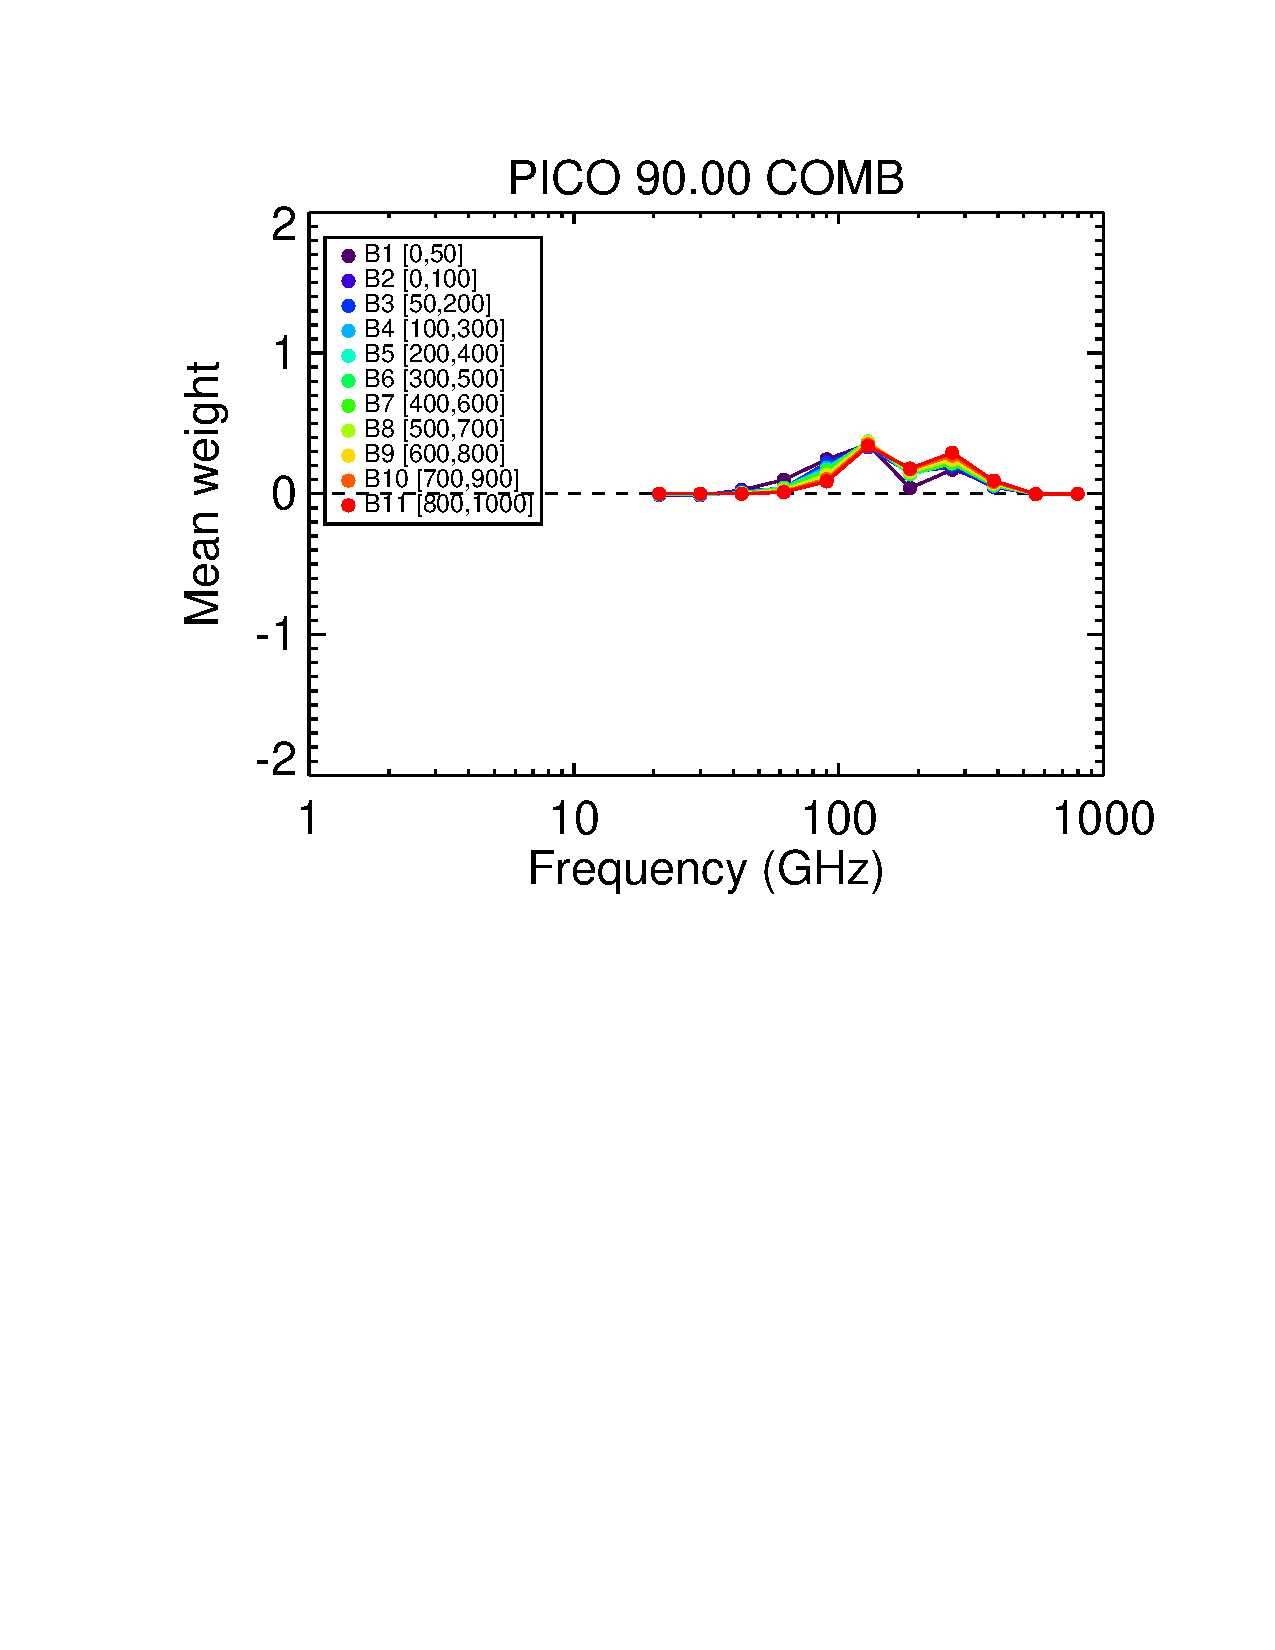
\includegraphics[width=0.6\textwidth,angle=0]{images/bsky_pico_comb_90.00_mean_weight3.pdf}
\hskip-5ex
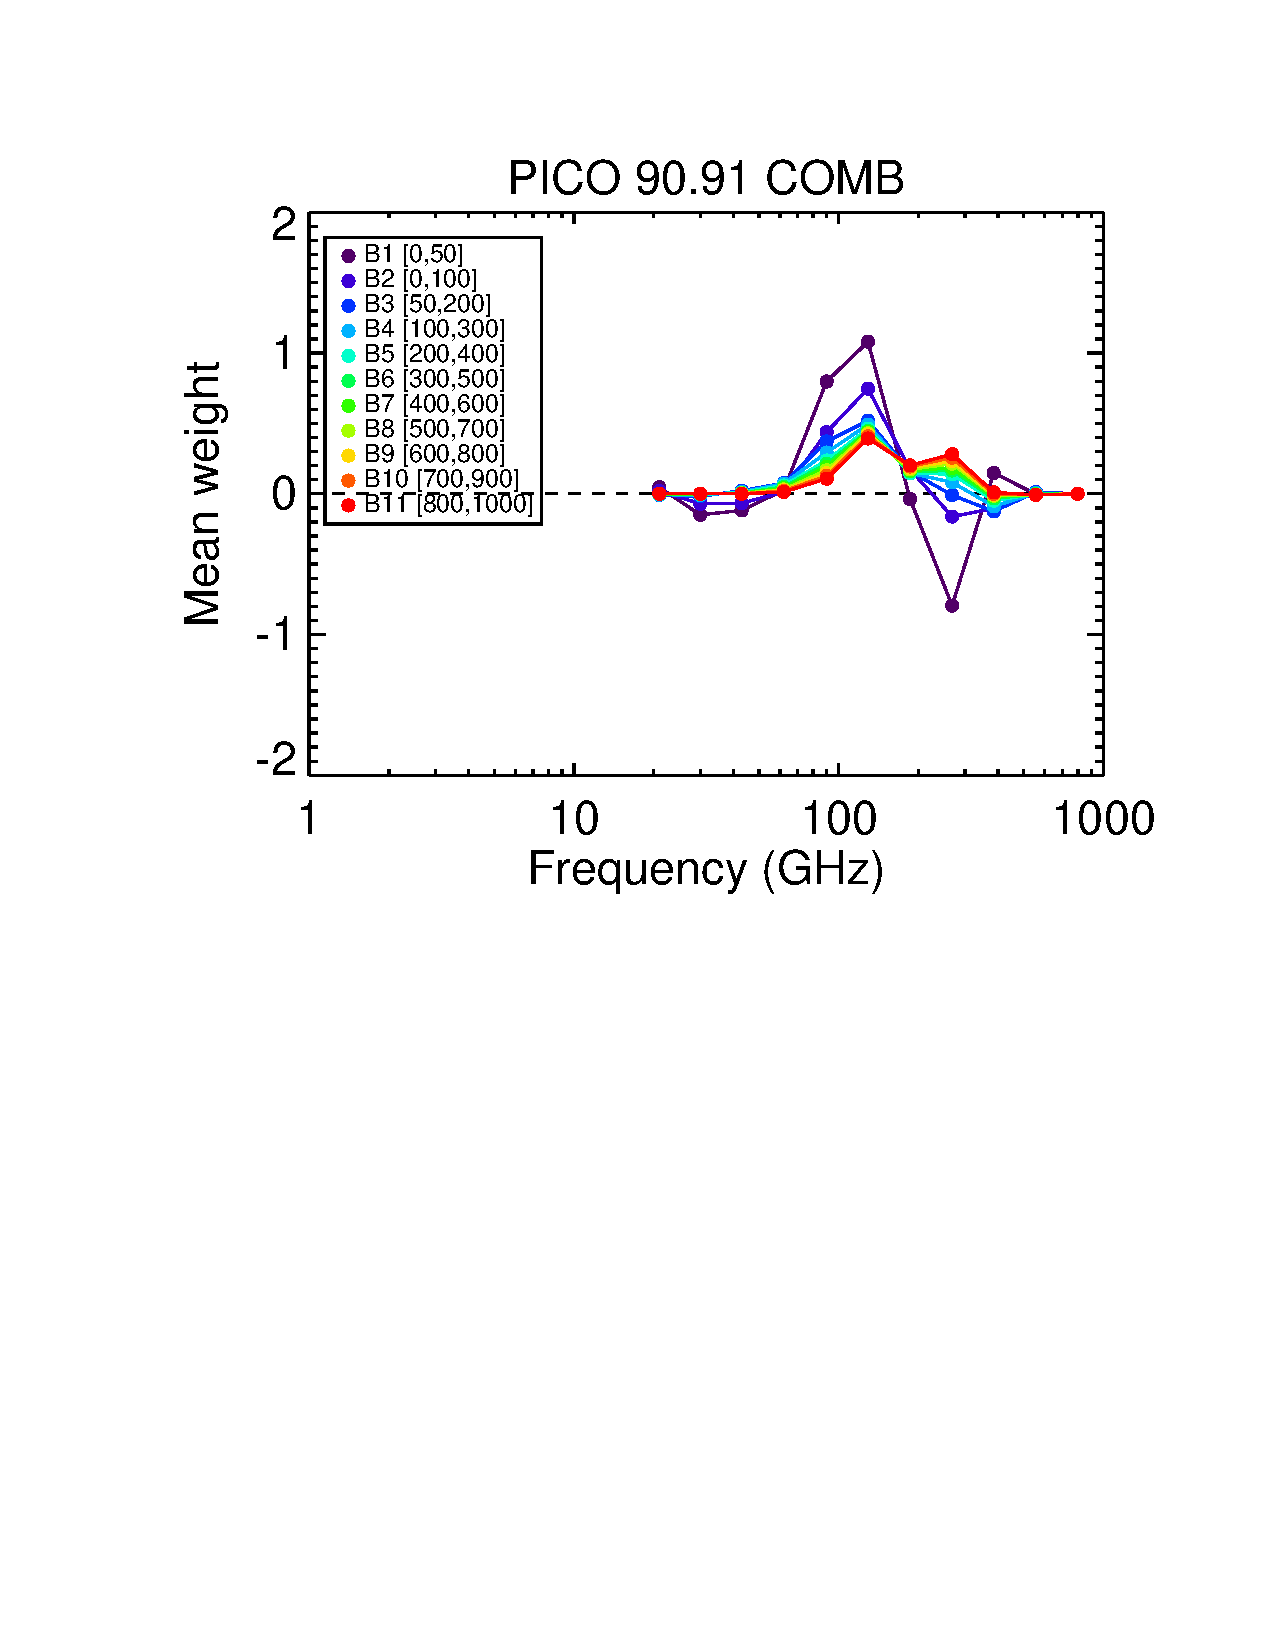
\includegraphics[width=0.6\textwidth,angle=0]{images/bsky_pico_comb_90.91_mean_weight3.pdf}
\vskip-25ex
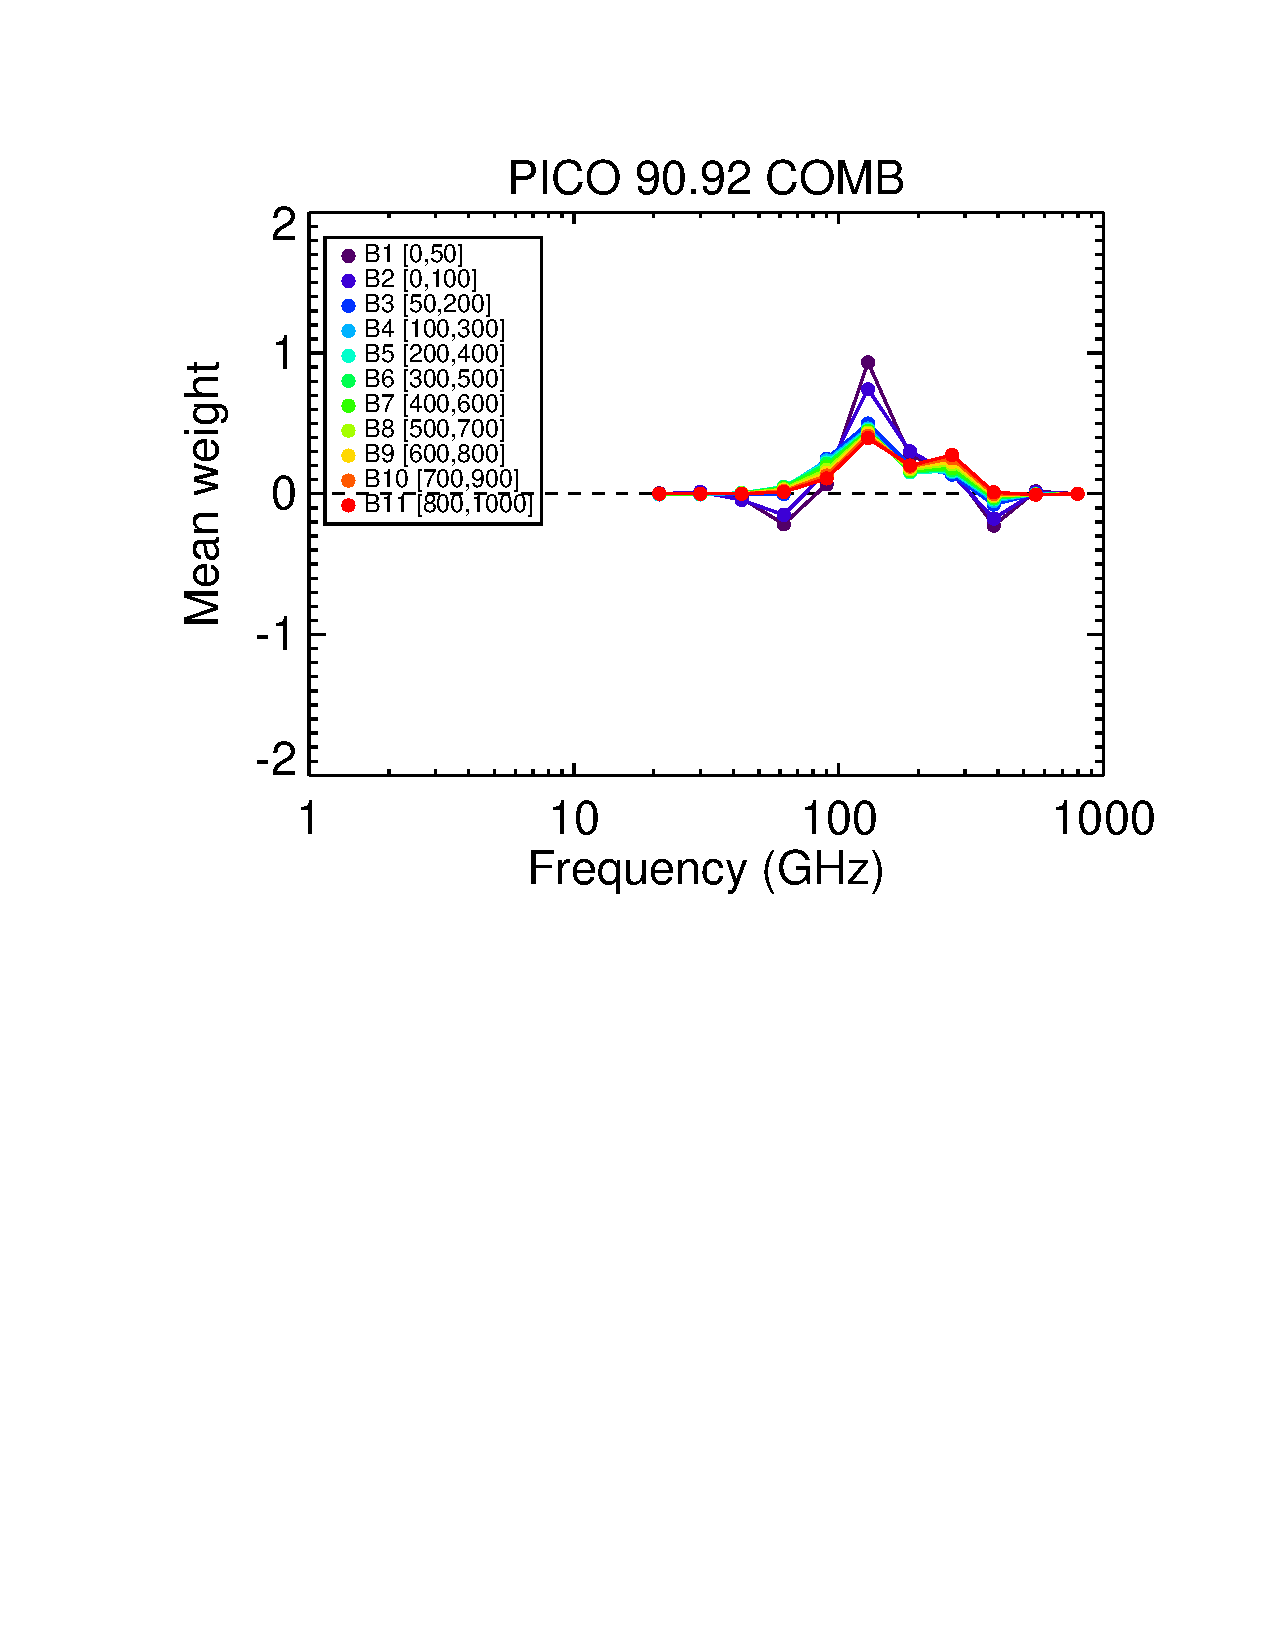
\includegraphics[width=0.6\textwidth,angle=0]{images/bsky_pico_comb_90.92_mean_weight3.pdf}
\hskip-5ex
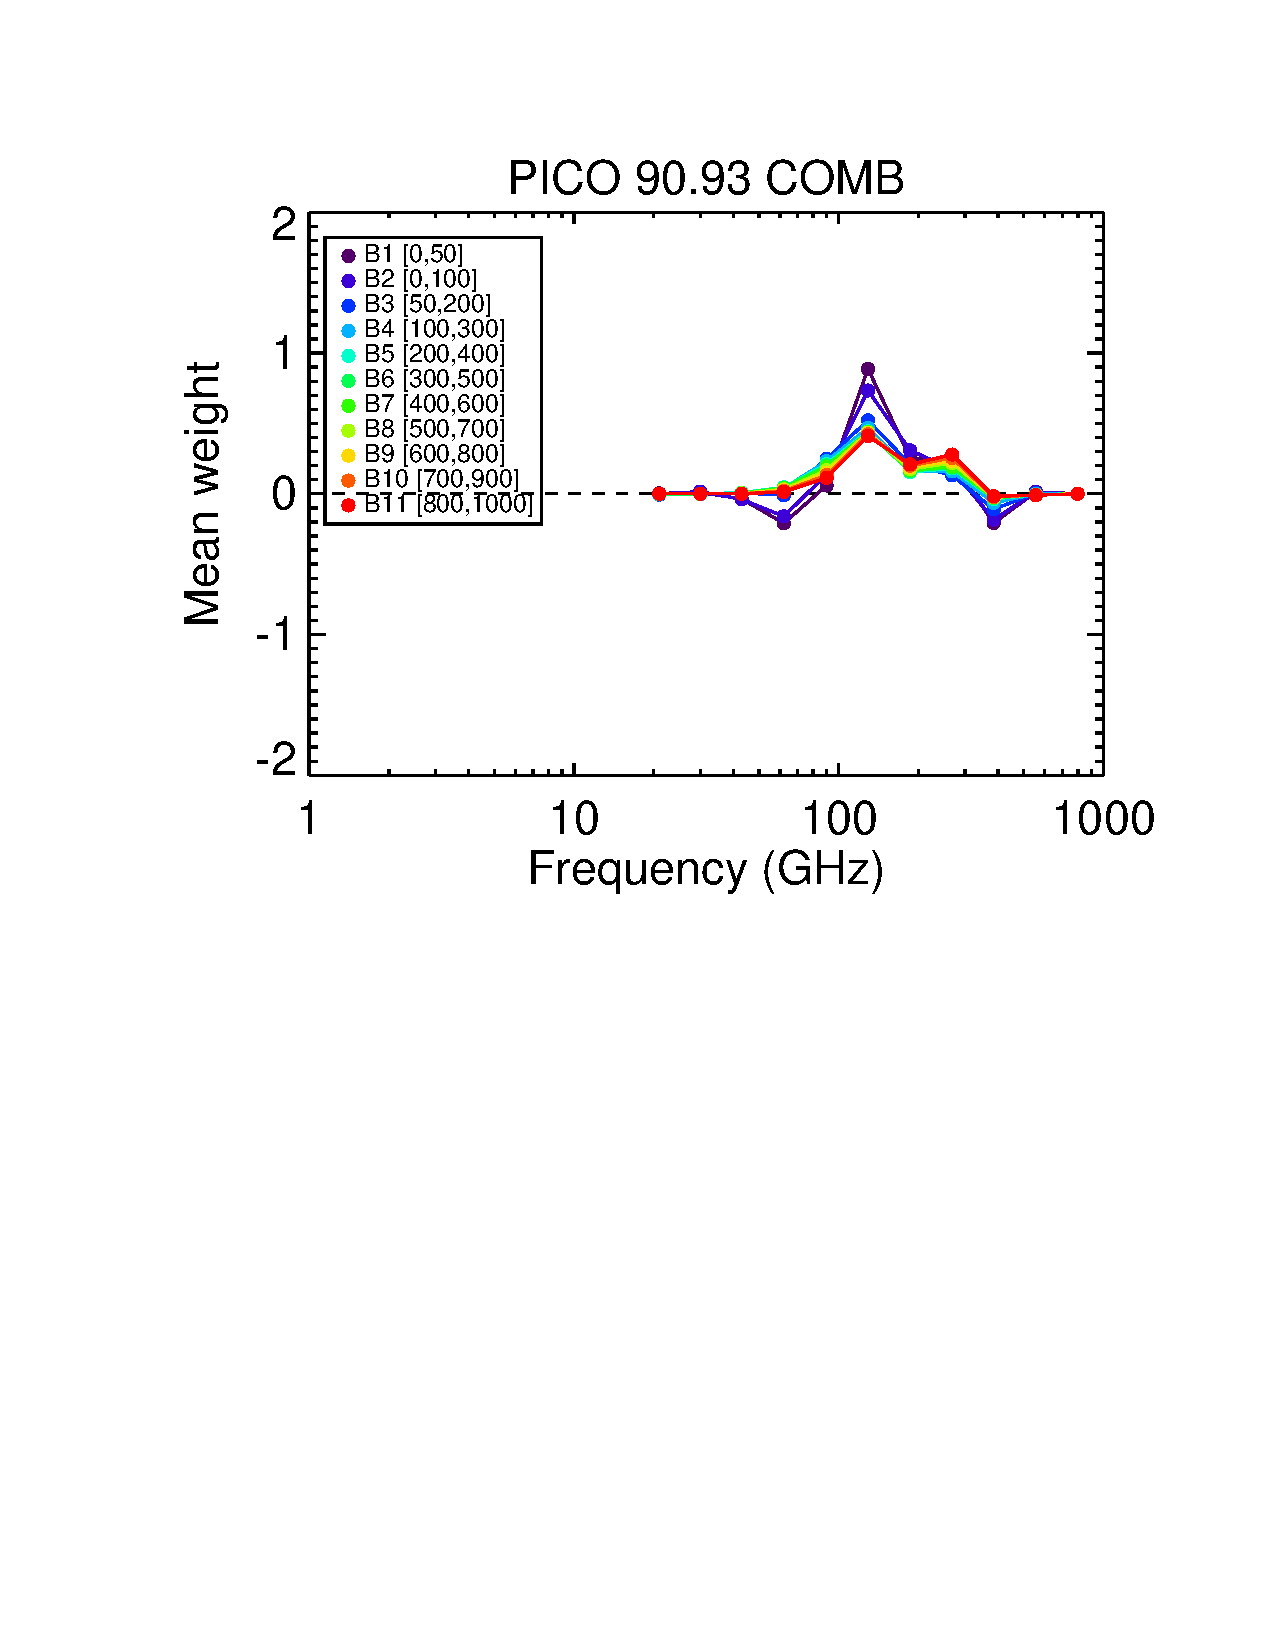
\includegraphics[width=0.6\textwidth,angle=0]{images/bsky_pico_comb_90.93_mean_weight3.pdf}
\vskip-25ex
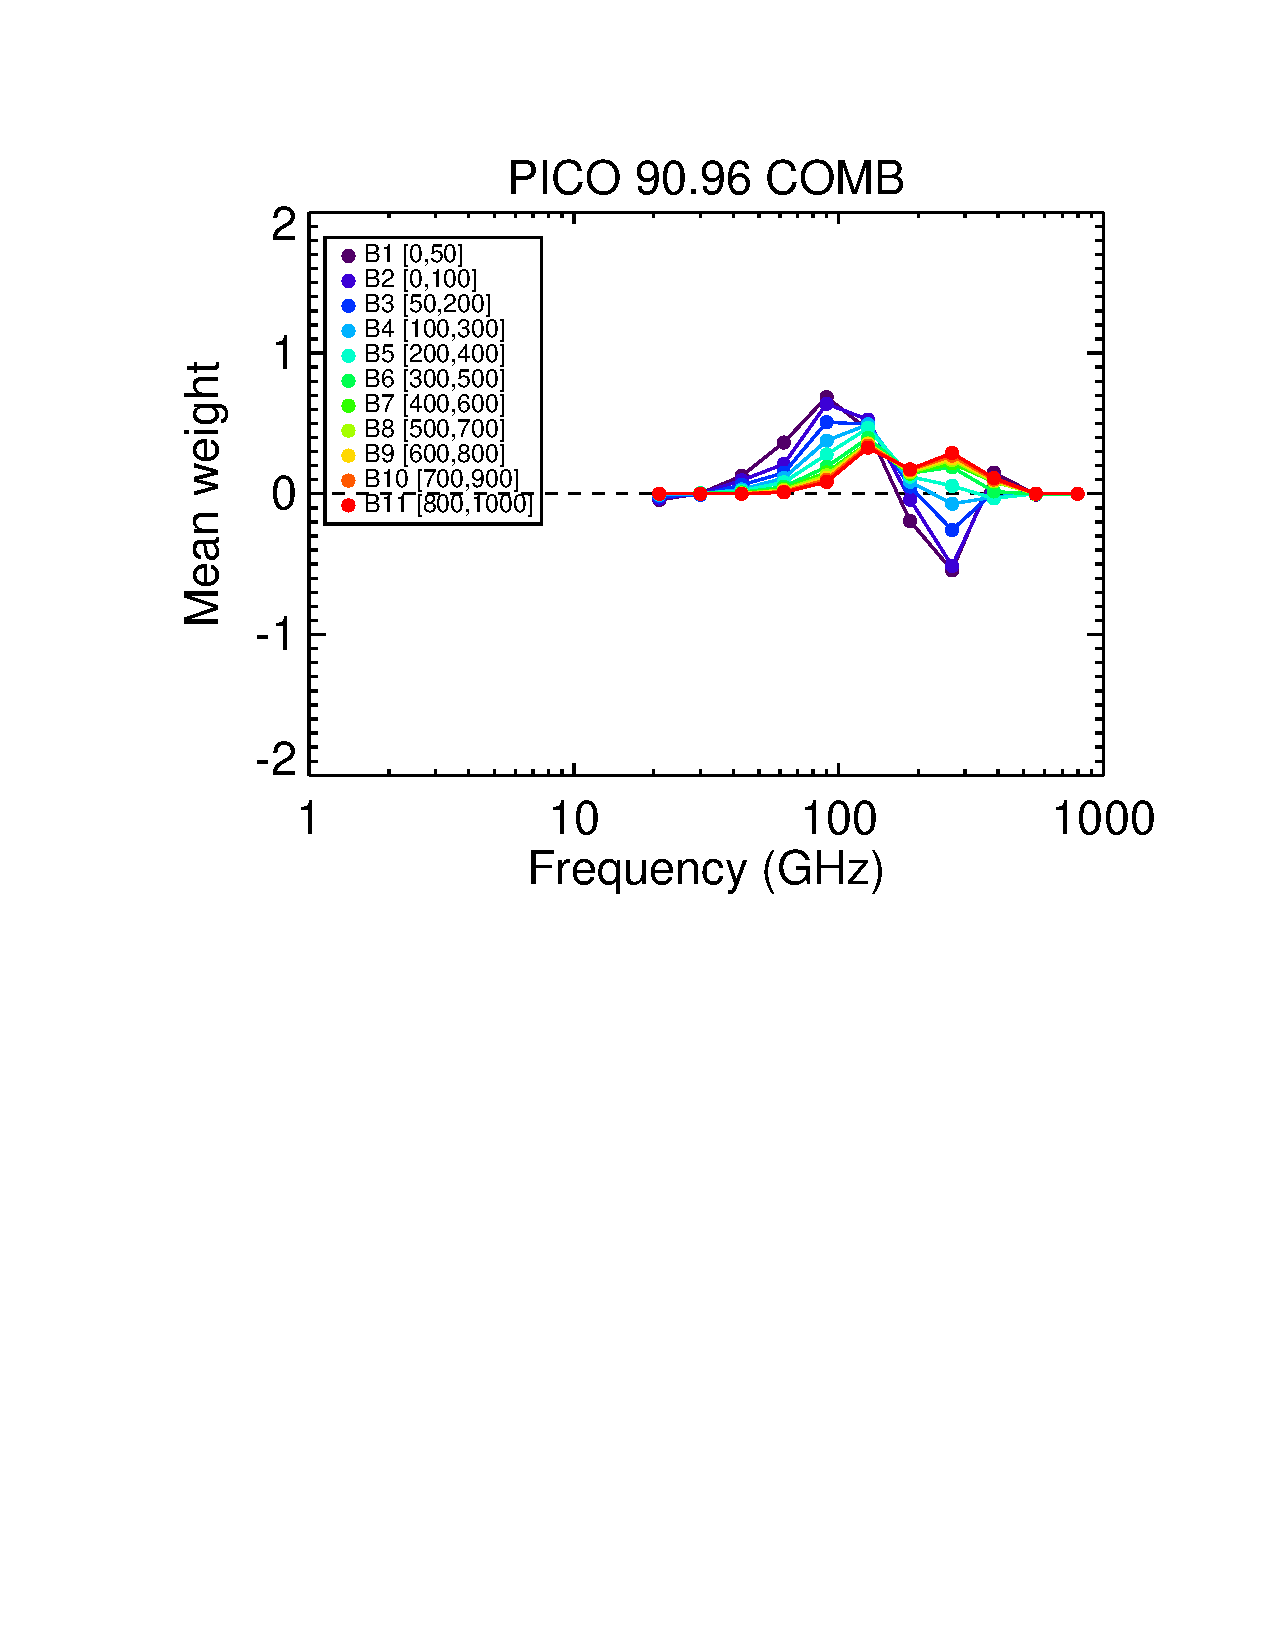
\includegraphics[width=0.6\textwidth,angle=0]{images/bsky_pico_comb_90.96_mean_weight3.pdf}
\hskip-5ex
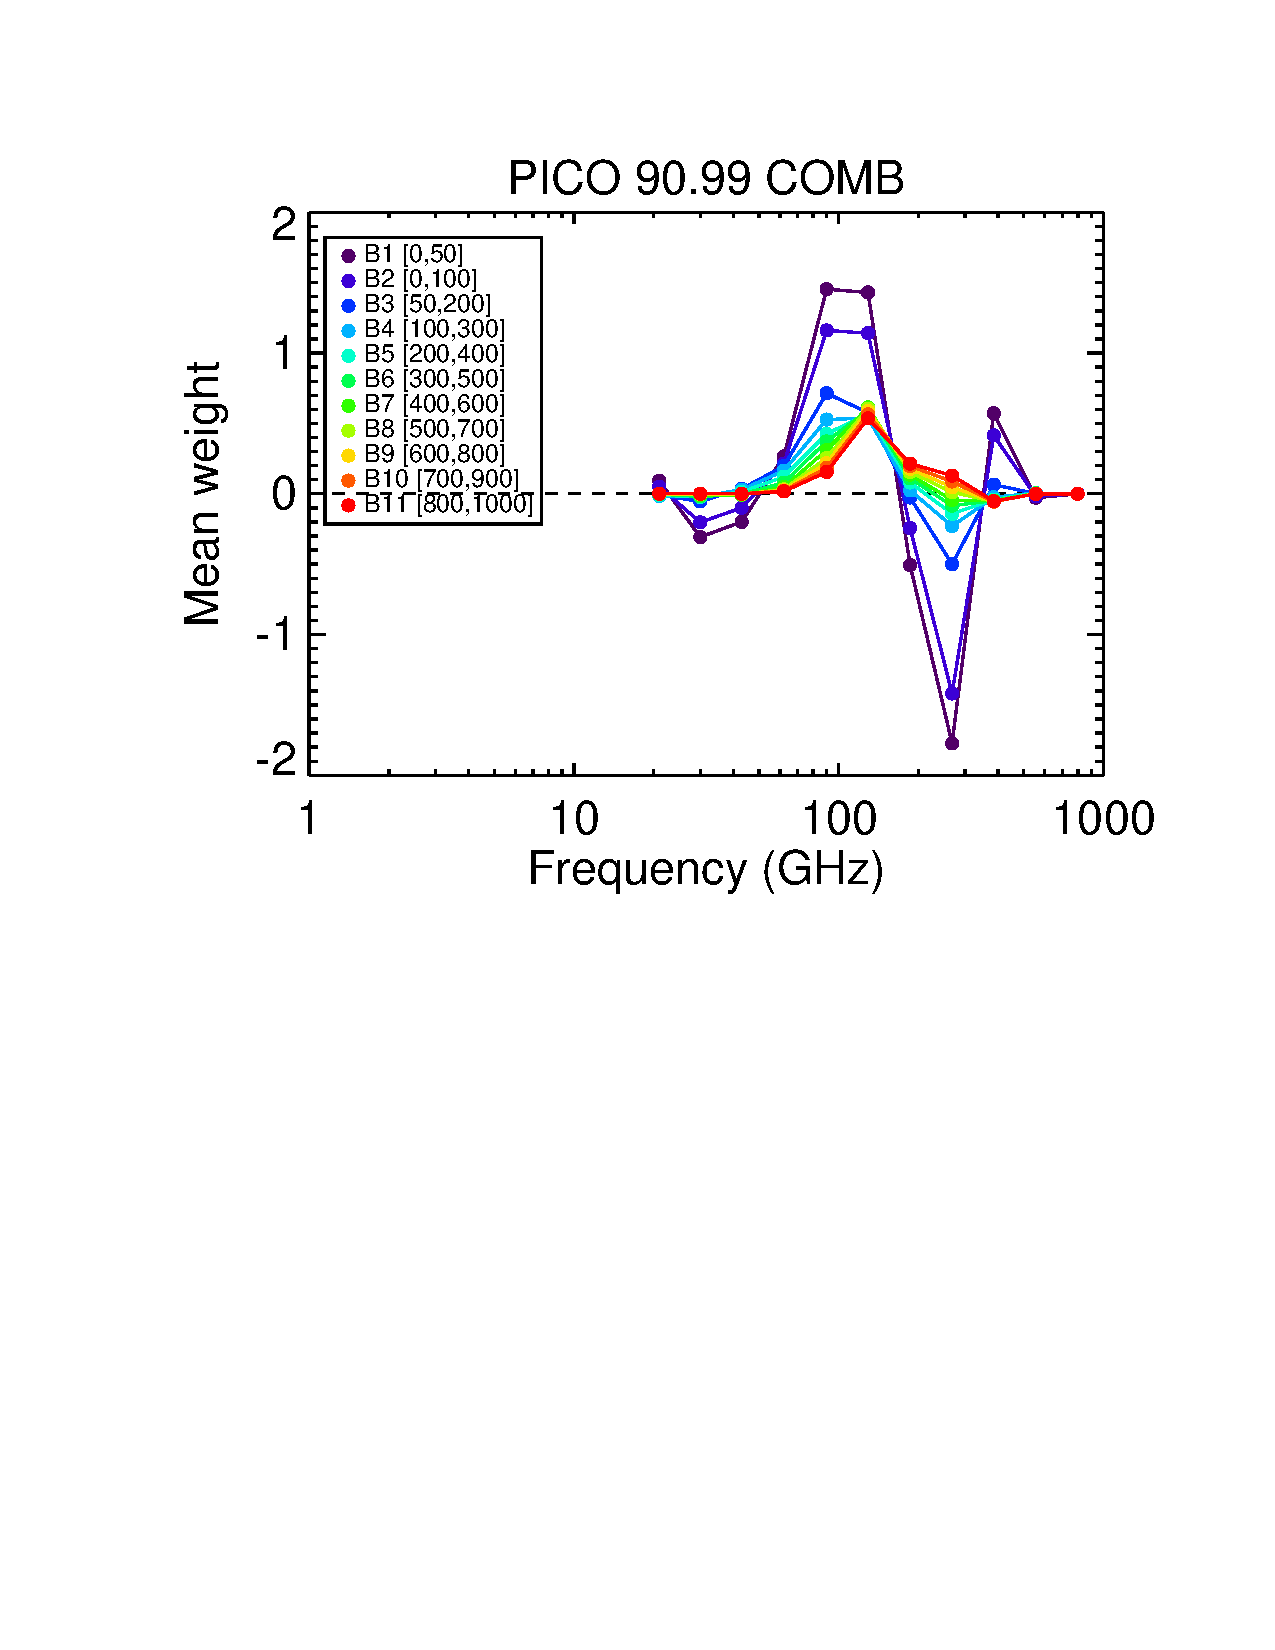
\includegraphics[width=0.6\textwidth,angle=0]{images/bsky_pico_comb_90.99_mean_weight3.pdf}
\end{figure}


\end{document}

%\begin{figure}[!htb]
%\centering
%
\includegraphics[width=4cm]{images/example}
%\caption{example}
%\label{fig:im_3}
%\end{figure}
